\documentclass[11pt]{article}
\usepackage{a4wide}
\usepackage[small,bf,hang]{caption}

\usepackage{amsmath}%nodig om zelf math operator te kunnen definiëren
\DeclareMathOperator{\Ker}{Ker}
\DeclareMathOperator{\Span}{span}
\DeclareMathOperator{\spoor}{sp}

\usepackage{amssymb}%nodig om mathbb te kunnen gebruiken, bijvoorbeeld voor verzameling van reële getallen

\usepackage[dutch]{babel}
\usepackage{graphicx}
\usepackage{float}
\usepackage{fancyhdr}

\graphicspath{{./images/}}
\setlength{\parindent}{0pt}%zorgt ervoor dat er niet wordt ingesprongen in het begin van een alinea

\renewcommand{\labelitemi}{$\triangleright$} 

%héél schoon lettertype :-)
\renewcommand*\rmdefault{ppl}

\usepackage{pdfpages}

%\newcommand{\mx}[1]{\ensuremath{\mathsf{#1}}}%matrix in juiste lettertype

\graphicspath{{./images/}}


%\pagestyle{fancy}
%\lhead{\textbf{NAAM:}}
%\renewcommand{\headrulewidth}{0pt}
%\chead{}
%\rhead{2011-2012}
%\lfoot{KAHO Sint-Lieven }
%\cfoot{Departement Industrieel Ingenieur}
%\rfoot{\thepage}

%ACHTERGROND
%\usepackage{eso-pic} \newcommand\BackgroundPic{ \put(0,0){  \parbox[b][\paperheight]{\paperwidth}{% %\vfill %\centering \includegraphics[height=29.7cm, keepaspectratio]{nietjeNietLosmaken.png}% %\vfill }}}

%Hoofdstuk 6. Wiskundige formules 79 6.5 Conventies voor matrices en vectoren
\newcommand{\vt}[1]{\ensuremath{\boldsymbol{#1}}} % vector in juiste lettertype
\newcommand{\mx}[1]{\ensuremath{\mathsf{#1}}} % matrix in juiste lettertype
\newcommand{\norm}[1]{\lVert #1 \rVert} %eigen commando voor de aanduiding van de norm met dubbele verticale lijnen
\newcommand{\absolutewaarde}[1]{\lvert #1 \rvert} %eigen commando voor de aanduiding van de absolute waarde met enkele verticale lijnen
\renewcommand{\labelitemi}{$\triangleright$}%aanpassing van de 'bullets' van 'itemize'

%BLANCO PAGINA INVOEGEN:
%\newpage
%\thispagestyle{empty} %The usage of \thispagestyle is \thispagestyle{option}. The option can be: plain - Just a plain page number. empty - Produces empty heads and feet - no page numbers. headings - Puts running headings on each page. The document style specifies what goes in the headings. myheadings - You specify what is to go in the heading with the \markboth or the \markright commands.
%\mbox{} %The major part is \mbox{}, which ensures the existence of an empty page.-

\title{\textbf{Het mysterie van de Wii Controller}}
%\subtitle{test}
\author {Dimitri Coppens}
\date{\today}

\begin{document}
\maketitle

\begin{flushright}Een workshop voor de leerlingen van Sint-Pieters,\\
gebaseerd op het werk van Geert Callebaut,\\
die zijn werk baseerde op dat van Johnny Chung Lee	
\end{flushright}

\begin{figure}[h]
\begin{center}
\includegraphics[width=155mm]{esmerelda.jpg}
\end{center}
\end{figure}

\newpage

\section{Maak zelf je digitale pen}
\vspace{3cm}
\begin{figure}[h]
\begin{center}
\includegraphics[width=17cm]{montageInfraroodPen.jpg}
\end{center}
\end{figure}

\newpage
\section{De Wii Controller ontmanteld: gebruikte technologie}

\begin{figure}[h] \begin{center}
\includegraphics[width=7cm]{newYorkTimesWiiController01.jpg}
\caption{[...]Beneath the controller's white plastic shells are an array of time tested digital technologies working together in new ways[...] \textit{bron:} "At the heart of the Wii, Micron-Size Machines," M. Marriott, The New York Times, December 21, 2006]}
\end{center} \end{figure}

\subsection{Functionality, Sensing}

%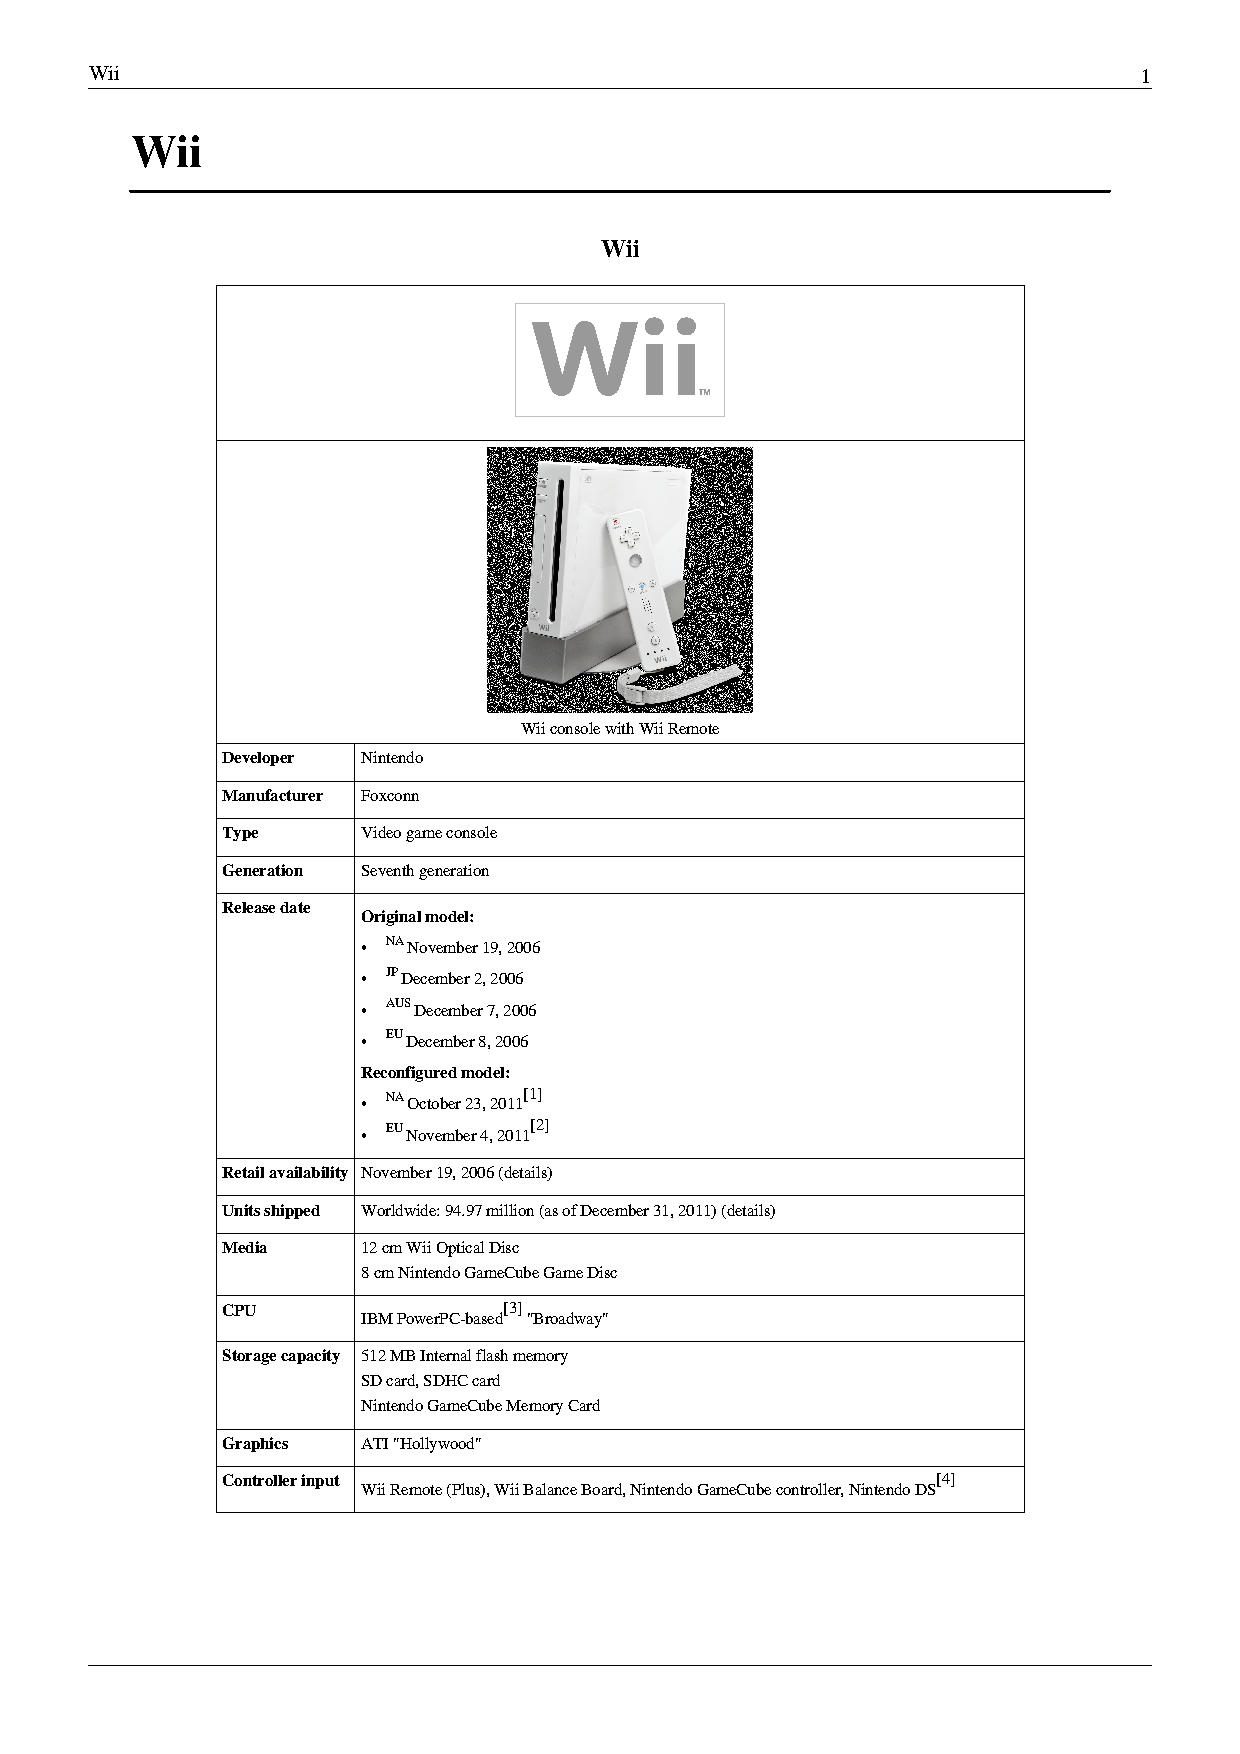
\includepdf[pages={1,2}]{wikipediaWii.pdf}

\begin{flushright}\textit{tekst gebaseerd op Wikipedia} \end{flushright} 
The Wii Remote has the ability to sense acceleration along three axes through the use of anaccelerometer. The Wii Remote also features an optical sensor, allowing it to determine where the Wii Remote is pointing. 

\begin{figure}[h]
\begin{center}
\includegraphics[width=7cm]{wiiControllerSchets.jpg}
\caption{Accelerometers behoren tot de `MEMs,´ de Micro-Electro-Mechanical systems}
\end{center}
\end{figure}

\newpage

The Sensor Bar is features ten infrared LEDs, five at each end of the bar. The LEDs furthest from the center are pointed slightly outwards, the LEDs closest to the center are pointed slightly inwards, while the rest are pointed straight forward. The bar may be placed above or below the television, and should be centered. If placed above, the sensor should be in line with the front of the television, and if placed below, should be in line with the front of the surface the television is placed on. It is not necessary to point directly at the Sensor Bar, but pointing significantly away from the bar will disrupt position-sensing ability due to the limited viewing angle of the Wii Remote. (volgens John Chung Lee = 45 graden?)\\

Use of the Sensor Bar allows the Wii Remote to be used as an accurate pointing device up to 5 meters (approx. 16 ft) away from the bar. The Wii Remote's image sensor is used to locate the Sensor Bar's points of light in the Wii Remote's field of view. 
\begin{figure}[h]
\begin{center}
\includegraphics[width=10cm]{newYorkTimesWiiController02.jpg}
\caption{[bron: "At the heart of the Wii, Micron-Size Machines," M. Marriott, The New York Times, December 21, 2006]}
\end{center}
\end{figure}

\newpage
%wiiControllerSchetsOpticalSensor1.jpg
\subsection{Triangulatie met behulp van de sensor bar}
\begin{figure}[h]\begin{center}
\includegraphics[width=10cm]{wiiGebruikteTechnologie.jpg}
\caption{Met behulp van traingulatie berekent de controller haar positie t.o.v. de LED lampen en de hoek die ze maakt met de horizontale. De controller communiceert met de console via Bluetooth, die op haar beurt een WiFi verbinding tot stand kan brengen met het internet.}
\end{center} \end{figure}


The light emitted from each end of the Sensor Bar is focused onto the image sensor which sees the light as two bright dots separated by a distance "mi" on the image sensor. The second distance "m" between the two clusters of light emitters in the Sensor Bar is a fixed distance. From these two distances m and mi, the Wii CPU calculates the distance between the Wii Remote and the Sensor Bar using triangulation. 

\begin{figure}[h] \begin{center}
\includegraphics[width=8cm]{wiiControllerSchetsOpticalSensor1.jpg}
\end{center} \end{figure}

In addition, rotation Wii Remote 7 of the Wii Remote with respect to the ground can also be calculated from the relative angle of the two dots of light on the image sensor. Games can be programmed to sense whether the image sensor is covered, which is demonstrated in a Microgame of Smooth Moves, where if the player does not uncover the sensor, the champagne bottle that the remote represents will not open.

\begin{figure}[h]\begin{center}
\includegraphics[width=8cm]{wiiControllerSchetsOpticalSensor2.jpg}
\end{center}\end{figure}

The Sensor Bar is required when the Wii Remote is controlling up-down, left-right motion of a cursor or reticle on the TV screen to point to menu options or objects such as enemies in first-person shooters. \textbf{Because the Sensor Bar also allows the Wii Remote to calculate the distance between the Wii Remote and the Sensor Bar, the Wii Remote can also control \textit{slow} forward-backward motion of an object in a 3-dimensional game. \textit{Rapid} forward-backward motion, such as punching in a boxing game, is controlled by the acceleration sensors. Using these acceleration sensors (acting as tilt sensors), the Wii Remote can also control rotation of a cursor or other objects.}\\

The use of an infrared sensor to detect position can cause some detection problems when other infrared sources are around, such as incandescent light bulbs or candles. This can be easily alleviated by using fluorescent lights around the Wii, which emit little to no infrared light. \textbf{Innovative users have used other sources of IR light as Sensor Bar substitutes such as a pair of flashlights and a pair of candles. Such substitutes for the Sensor Bar illustrate the fact that a pair of non-moving lights provide continuous calibration of the direction that the Wii Remote is pointing and its physical location relative to the light sources.} There is no way to calibrate the position of the cursor relative to where the user is pointing the controller without the two stable reference sources of light provided by the Sensor Bar or substitutes. \\

\newpage

\subsection{Light Emitting Diode}

\begin{figure}[h]
\begin{center}
\includegraphics[width=10cm]{giancoli_2_p1257.jpg}
\caption{[bron: Giancoli]}
\end{center}
\end{figure}

\begin{figure}[h]
\begin{center}
\includegraphics[width=5cm]{schemaLedWikipedia.jpg}
\caption{Bron: wikipedia[bron: Wikipedia]}
\end{center}
\end{figure}

\begin{figure}[h]
\begin{center}
\includegraphics[width=5cm]{wikipediaChemieLed.png}
\caption{Bron: wikipedia[bron: Wikipedia]}
\end{center}
\end{figure}

\newpage

\subsection{Draadloze Communicatie}

\begin{figure}[h]
\begin{center}
\includegraphics[width=5cm]{inDeGloriaDenDraad.jpg}
\caption{Niet alle draden zijn zichtbaar [uit: 'In de Gloria']}
\end{center}
\end{figure}

\subsubsection{Infrarood}


\textbf{Wikipedia: Infrared Photography - Digital cameras} \\

In infrared photography, the film or image sensor used is sensitive to infrared light. The part of the spectrum used is referred to as near-infrared to distinguish it from far-infrared, which
is the domain of thermal imaging. Wavelengths used for photography range from about 700 nm to about 900 nm. \\
... \\
Digital camera sensors are inherently sensitive to infrared light,[15] which would interfere with the normal photography by confusing the autofocus calculations or softening the image (because infrared light is focused differently from visible light), or oversaturating the red channel. Also, some clothing is transparent in the infrared, leading to unintended (at least to the manufacturer) uses of video cameras. Thus, to improve image quality and protect privacy, many digital cameras employ infrared blockers. Depending on the subject matter, infrared photography may not be practical with these cameras because the exposure times become overly long, often in the range of 30 seconds, creating noise and motion blur in the final image. However, for some subject matter the long exposure does not matter or the motion blur effects actually add to the image. Some lenses will also show a 'hot spot' in the centre of the image as their coatings are optimised for visible light and not for IR.\\

\textbf{'maak zelf je infrarode camera'}

\begin{figure}[h]
\begin{center}
\includegraphics[width=155mm]{emGolf.jpg}
\caption{Een elektrisch veld wordt opgewekt door een veranderend magnetisch veld, een magnetisch veld door veranderend elektrisch veld (of door een elektrische stroom)}
\end{center}
\end{figure}


\begin{figure}[h]
\begin{center}
\includegraphics[width=155mm]{golflengtes.jpg}
\caption{Verschillende families EM golven op basis van golflengte of frequentie}
\end{center}
\end{figure}

\subsubsection{Bluetooth}

\textbf{Wikipedia - Bluetooth}\\
Bluetooth is a proprietary open wireless technology standard for exchanging data over short distances (using short wavelength radio transmissions in the ISM band from 2400-2480 MHz) from fixed and mobile devices, creating personal area networks (PANs) with high levels of security. [...] It can connect several devices, overcoming problems of synchronization.
\\
Bluetooth uses a radio technology called frequency-hopping spread spectrum, which chops up the data being sent and transmits chunks of it on up to 79 bands (1 MHz each; centered from 2402 to 2480 MHz) in the range 2,400-2,483.5 MHz (allowing for guard bands). This range is in the globally unlicensed Industrial, Scientific and Medical (ISM) 2.4 GHz short-range radio frequency band.

\subsubsection{Wi-Fi}




\subsection{Accelerometers en Micro-Electro-mechanical system}

\begin{flushright}[...]The controller's most-talked feature is the capacity to track it's own relative motion[...] \textit{bron:} "At the heart of the Wii, Micron-Size Machines," M. Marriott, The New York Times, December 21, 2006]
\end{flushright}

(Ook gebruikt voor activatie air-bag.)
\\

But the controller's most-talked-about feature is the capacity to track its own relative motion. This enables players to do things like steer a car by twisting the remote in the air or moving a game character by tilting the remote down or up. `` This represents a fabulous example of the consumerization of MEMS, '' the tiny devices known as microelectro- mechanical systems, said Benedetto Vigna, general manager of the MEMS unit at STMicroelectronics, a leading maker of the accelerometers embedded in the controllers. (Nintendo itself declined to talk about the controller's inner workings.)\\

He said the motion sensors, using the technology that activates vehicle air bags, can accurately sense three axes of acceleration: up and down, left to right, and forward and backward. \\

This is mostly achieved within the MEMS, micron-size machines that depend on submicroscopic structures carved into the silicon. For example, one structure moves like a tiny diving board, stimulated by the actions of the game players.\\
 
The structures are enveloped in an electrical field, Mr. Vigna said. When the MEMS elements are moved, the electrical field changes and the MEMS chip is sensitive enough to detect the changes. \\

These accelerometers are so sensitive, Mr. Vigna said, because electrons --- those subatomic particles that whirl around the nucleus of atoms like a video game in the making --- can sense the subtle atomic-level movement of the silicon structures.\\

\textit{bron:} "At the heart of the Wii, Micron-Size Machines," M. Marriott, The New York Times, December 21, 2006]

\begin{figure}
\begin{center}
\includegraphics[width=10cm]{newYorkTimesWiiController03.jpg}
\caption{[...]MEMS are micron-sized machines that depend on submicroscopic structures carved into the silicon. For example, one structure moves like a tiny diving board, stimulated by the actions of the game players.[...] \textit{bron:} "At the heart of the Wii, Micron-Size Machines," M. Marriott, The New York Times, December 21, 2006]}
\end{center}
\end{figure}





\subsection{multitouch}



\section{Andere toepassingen van de Wii}
of: hoe een ind. ir. zich uitleeft op bestaande technologie
http://www.multiwii.com/
low-cost motion capturing using nintendo wii remote controllers

\section{Bronvermelding}

boekje van geert callebaut
http://www.nytimes.com/2006/12/21/technology/21howw.html?ref=technology

\includepdf[pages={1,2}]{newYorkTimes_atTheHeartOfTheWiiMicronSizeMachines.pdf}
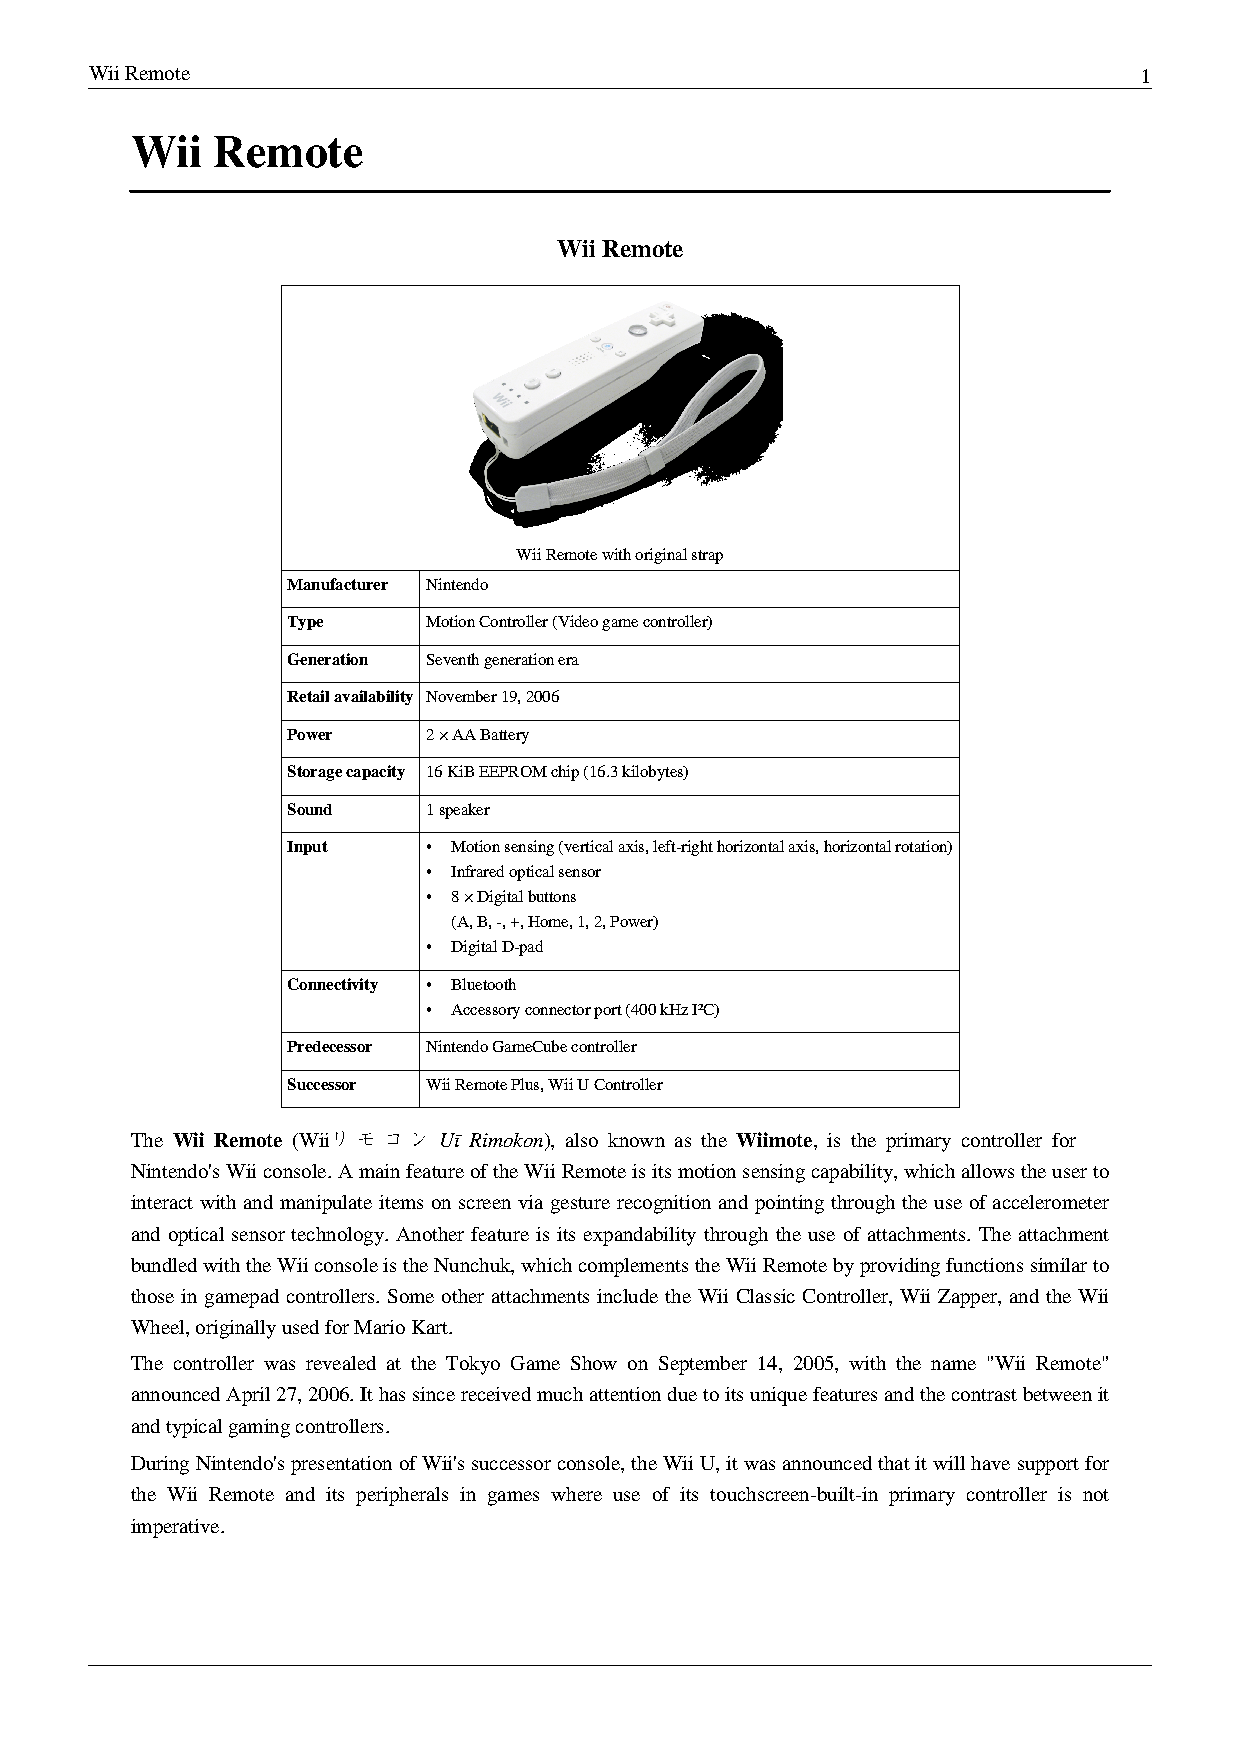
\includepdf[pages={1-13}]{wikipediaWiiController.pdf}


\end{document}